


%----------------------------------------------------------------------
\section{Paper's Content}
\textbf{Classical problem, history}
The task of labeling edges as convex, concave, and occluding entities~\cite{kanade1981recovery,Koenderink1984,lineCurvedObjects,mild-sugihara}
is one of the classical problems in computer vision. This problem was first addressed on synthetic drawings, where several 
constraint satisfaction algorithms were proposed~\cite{mild-sugihara}. On real image data, the problem of labeling 
line-drawings is a very hard problem. Furthermore, this problem was shown to be challenging even on RGBD data obtained 
using commodity sensors like Kinect. This paper studies the problem of classifying boundaries from RGBD data. 
One could also apply such techniques to dense point clouds computed using multiview 
techniques~\cite{furukawa-PAMI10,Snavely2006}. 
\begin{figure}[t]
\centering
       \subfigure[RGB Image]{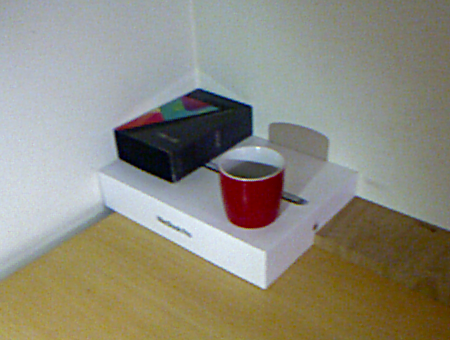
\includegraphics[width=0.32\columnwidth]{images/Im1-RGB.png}} \hfill
       \subfigure[Edge Types]{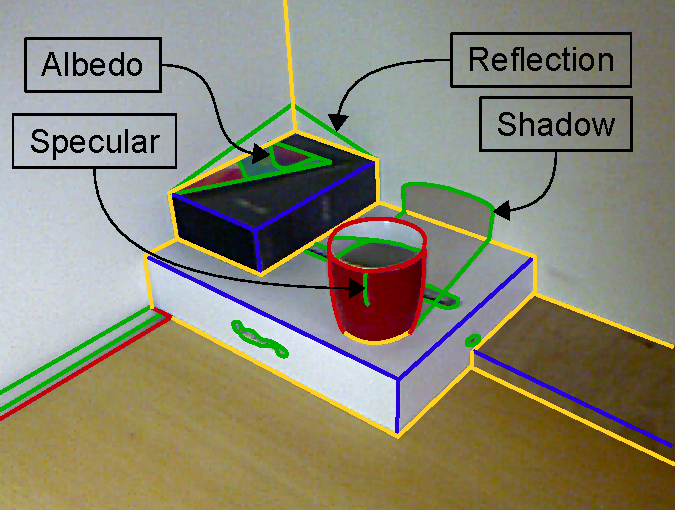
\includegraphics[width=0.32\columnwidth]{images/Im1-Labelled-1.pdf}} \hfill
       \subfigure[Depth Map]{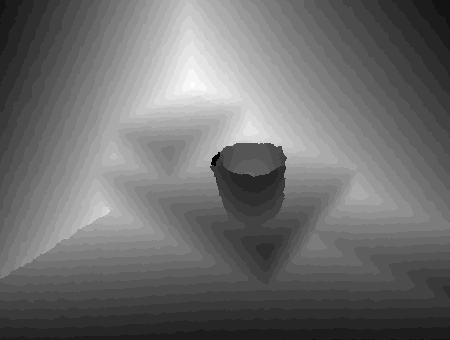
\includegraphics[width=0.32\columnwidth]{images/Im1-Depth.png}} \\
\caption{\it The edges in (a) are marked in (b) with the color code: red (occluding), green (planar),
blue (convex), and yellow (concave). Planar edges are caused by different phenomena as marked.
(c) shows the Kinect depth map (note the depth quantization artifacts).}
\label{fig:EdgeLabeling}
\end{figure}	

\textbf{Edges}
Edges in an image often correspond to depth discontinuities at object boundaries (occlusion 
edges) or normal discontinuities (convex or concave edges). In addition, there could be 
planar edges that are within planar regions. Figure~\ref{fig:EdgeLabeling} shows an image 
containing different types of edges. Note that planar edges may result from shadows, reflection, 
specularities and albedo variations. In classical line labeling with synthetic line 
drawings, we do not have any planar edges as the purpose of edge labeling has always been to 
classify the depth edges into occluding, convex and concave entities. However, in real images planar 
edges occur more frequently than others. 

\textbf{importance, applications (reconstruction, segmentation and recognition, challenges}
Contours are critical to the human perception of scenes. Beyond localizing the discontinuities 
in the color distribution, edges provide cues related to the surface orientation and depth 
discontinuities. The importance of edges in understanding of structure was realized quite 
early with works on recovering 3D structure from single 
 images~\cite{malik1989recovering,kanade1981recovery}. Hoiem \textit{et al.}~\cite{hoiem-ROB} showed that occlusion boundaries provide very useful cues to estimate the depth of a scene from a single image. It was shown that PMVS 
point cloud~\cite{furukawa-PAMI10} can be densified and improved if occluding contour information 
is available~\cite{qishan2014Occluding}. In our work, we specifically focus on providing this
information. Two important challenges need to be addressed in order to use this information in a 
recognition or reasoning algorithm. The first arises from the incompleteness of edge information 
derived from real-world images as well as noisy edges from lighting and other imaging conditions. 
The second is due to inherent ambiguities in mapping from edges to structure, where the same 
edge map can result from multiple object configurations~\cite{mild-sugihara}. As a result, many existing 
algorithms~\cite{gcontext-hoiem,hedau2012,schwing2012b,Lifting3DManhattan,lee2010} use the boundary 
pixels for semantic labeling and depth estimation without considering the class labels for these edge pixels. 

\textbf{Close relation with Jia et al}
Our approach is closely related to the work of Jia \textit{et al.}~\cite{depthorder}. The main 
similarity is the use of a 2D MRF to infer the edge labels. However, there are many other 
differences. Jia \textit{et al.}~\cite{depthorder} showed three-class labeling of occluding, connecting and 
homogeneous boundaries from RGBD data. On the contrary, we show four class edge labeling. In their 
approach, plane-fitting near edges are used to compute the features for the task of edge-labeling. 
In their approach, SVM regression is used for unary feature computation, whereas we use Random 
forest. In our work, we rely on simple depth comparison features for the classification and such simple 
features are more robust to missing data and noise in comparison to plane fitting techniques. Note that 
such simple edge comparison features are shown be useful in Kinect human pose regression work of 
Shotton \textit{et al.}~\cite{newcombe2011kinectfusion}.

\textbf{Gupta et al}
Gupta \textit{et al.}~\cite{gupta13Perceptual} addressed the problem of indoor scene understanding
from a single RGBD image, where they segment and classify image regions. In the process, they also 
label the edges to be convex, concave or occluding, and provide some qualitative results of the same. 
We are interested in classifying every edge pixel as one of the four types: convex, concave,
occluding and planar. We use the local information available from color, depth and surface
normals for this purpose. Our experiments show that we perform better than 
Gupta \textit{et al.}~\cite{gupta13Perceptual}.

\textbf{RGB is being explored. Why RGBD ?}
There has been a few methods that address the edge labeling from single RGB images. 
Fouhey \textit{et al.}~\cite{Fouhey14c} addressed this problem in an indoor Manhattan world setting, 
while Gupta \textit{et al.}~\cite{Fouhey14c} and Eigen \textit{et al.}~\cite{Eigen2014} predict normal 
and depth maps respectively from a single view using deep networks, which can then be used for 
detecting and labeling edges. 
We solve the problem using coarse depth information. In many 3D models obtained using RGBD sensors 
or multi-view reconstruction techniques, we typically have very noisy 3D point cloud near the 
boundaries. This is because most stereo reconstruction algorithms and structured light techniques 
are known to provide noisy reconstruction near the boundaries. For example, the accuracy of 3D 
points obtained from a Kinect sensor is extremely noisy near the boundaries. Thus the labeling 
problem that we address in this paper is not straightforward. We believe 
that by first solving this problem in RGBD settings, we will get the necessary insights to 
solve the more challenging problem of labeling edges from a single RGB image.

\section{Edges in scene understanding} 
\label{sec:SECTION1NAME}
%-------------------------------
History of edge labeling; applications like segmentation, reconstruction and recognition; importance of edge labels in understanding the scene; some papers; \\
~\cite{3dFromSingleView}
%----------------------------------------------------------------------
\section{Depth estimation techniques} 
\label{sec:SECTION2NAME}


%-------------------------------
\subsection{Monocular}
	
%------------------------------
\subsection{Stereo}


%--------------------------------
\subsection{3D scanner}
In many 3D models obtained using RGBD sensors or multi-view reconstruction techniques, we typically have very noisy 3D point cloud near the boundaries. This is because most stereo reconstruction algorithms and structured light techniques are known to provide noisy reconstruction near the boundaries.

~\cite{Authors06}

